%%%%%%%%%%%%%%%%%%%%% chapter.tex %%%%%%%%%%%%%%%%%%%%%%%%%%%%%%%%%
%
% sample chapter
%
% Use this file as a template for your own input.
%
%%%%%%%%%%%%%%%%%%%%%%%% Springer-Verlag %%%%%%%%%%%%%%%%%%%%%%%%%%
%\motto{Use the template \emph{chapter.tex} to style the various elements of your chapter content.}
\chapter{(Nice) Tree Decomposition}
\label{c:ntd} % Always give a unique label
% use \chaptermark{}

\section{Tree Decomposition}
\label{sec:ntd_td}
\begin{definition}
(Tree decomposition, \cite{robertson1984graph}). Eine Tree Decomposition \textit{eines (ungerichteten oder gerichteten) Graphen $G$ ist ein Baum $\mathbb{T}$ in dem jedem Knoten $x \in \mathbb{T}$ eine Menge von Knoten $B_x \subseteq V$ (genannt \glqq Bag\grqq) zugeordnet ist, so dass 
\begin{itemize}
\item für jede Kante $uv \in E$ existiert ein $x \in \mathbb{T} $, so dass $u,v \in B_x$
\item falls $v \in B_x$ und $v \in B_y$, dann $v \in B_z$ für alle $z$ auf dem Pfad von $x$ nach $y$ in $\mathbb{T}$
\end{itemize}
}
\end{definition}

Das Konzept der Tree Decomposition wurde 1976 von Rudolf Halin \cite{Halin1976} eingeführt. Sie dient dazu die Baumweite zu definieren und Berechnungsprobleme auf Graphen schneller zu lösen.

Die Baumweite ist eine Zahl und beschreibt die \glqq Baum-Ähnlichkeit\grqq ~eines Graphen. Die Baumweite $tw(\mathbb{T})$ einer Tree Decomposition $\mathbb{T}$ ist die Größe des größten Bags minus eins. Die Baumweite eines Graphen $G$ ist die minimale Baumweite aller möglichen Tree Decompositions von $G$.

Ein Beispiel für eine Tree Decomposition ist in Abbildung \ref{fig:td_2} gegeben. Der Ursprungsgraph ist in Abbildung \ref{fig:td_1}.

\begin{figure}
\centering
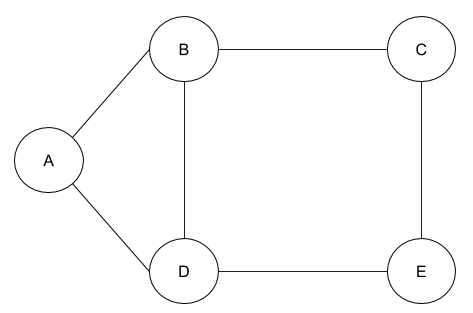
\includegraphics[width=0.5\textwidth]{./imgs/TD_1.png}
\caption{Ursprungsgraph für eine Tree Decomposition}
\label{fig:td_1}
\end{figure}

\begin{figure}
\centering
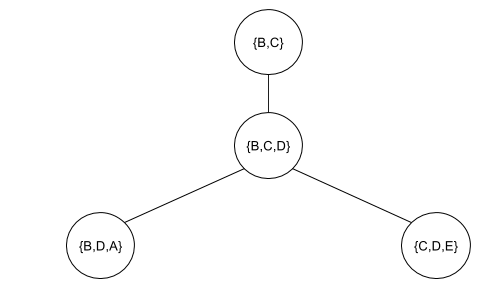
\includegraphics[width=0.6\textwidth]{./imgs/TD_2.png}
\caption{Eine Tree Decomposition für den in Abbildung \ref{fig:td_1} gegebenen Ursprungsgraphen}
\label{fig:td_2}
\end{figure}

\section{Nice Tree Decomposition}
\label{sec:ntd_ntd}
Kloks \cite{kloks1994} führte die sogenannte Nice Tree Decomposition ein, welche oft für Algorithmen mit dynamischen Programmen genutzt werden. Da in Sektion \ref{sec:ntd_req} weitere Modifikationen auf Basis der Nice Tree Decomposition eingeführt werden, wird die hier vorgestellte Nice Tree Decomposition als \textit{standardmäßige Nice Tree Decomposition} bezeichnet.

\begin{definition}
Eine standardmäßige Nice Tree Decomposition ist eine \textit{Tree Decomposition, für die gilt:
\begin{itemize}
\item jeder Bag besitzt höchstens zwei Kind-Knoten
\item falls ein Bag $x$ zwei Kind-Knoten $l,r$ besitzt, dann gilt $B_x=B_l=B_r$
\item falls ein Bag $x$ einen Kind-Knoten besitzt, dann gilt entweder $|B_x|=|B_y| + 1$ und $B_y \subseteq B_x$ oder $|B_x| + 1 = |B_y|$ und $B_x \subseteq B_y$
\end{itemize}
}
\end{definition}

\section{Weitere Modifikationen}
\label{sec:ntd_req}
Für den von \cite{cygan_solving_2011} beschriebenen Algorithmus wird die standardmäßige Nice Tree Decomposition zusätzlich noch auf folgende Weise modifiziert:
\begin{definition}
(Nice Tree Decomposition). Eine Nice Tree Decomposition \textit{ist eine Tree Decomposition mit einem speziellen Bag $z$ (Wurzel) mit $B_z=\emptyset$ und in der jeder Bag einer der folgenden Arten entspricht:
\begin{itemize}
\item \textbf{Leaf Bag}: ein Blatt $x$ aus $\mathbb{T}$ mit $B_x=\emptyset$ .
\item \textbf{Introduce Vertex Bag}: ein innerhalb von $\mathbb{T}$ liegender Knoten $x$ mit einem Kind-Knoten $y$ für den gilt $B_x=B_y \cup \{v\}$ für ein $v \notin B_y$. Dieser Bag führt den Knoten $v$ ein.
\item \textbf{Introduce Edge Bag}: ein innerhalb von $\mathbb{T}$ liegender Knoten $x$, der mit der Kante $uv \in E$ gekennzeichnet ist und einen Kind-Knoten $y$ mit $u,v \in B_x = B_y$ besitzt. Dieser Knoten führt die Kante $uv$ ein.
\item \textbf{Forget Bag}: ein innerhalb von $\mathbb{T}$ liegender Knoten $x$ mit einem Kind-Knoten $y$, für den gilt $B_x=B_y\backslash \{v\}$ für ein $v \in B_y$. Dieser Bag vergisst den Knoten $v$.
\item \textbf{Join Bag}: ein innerhalb von $\mathbb{T}$ liegender Knoten $x$ mit zwei Kind-Knoten $l,r$, für die $B_x=B_r=B_l$ gilt. 
\end{itemize}
Zusätzlich wird gefordert, dass jede Kante aus $E$ genau einmal eingeführt wird.
}\\

Ein Beispiel für eine Nice Tree Decomposition ist in Abbildung \ref{fig:td_3}.
\begin{figure}
\label{fig:td_3}

  \centering
    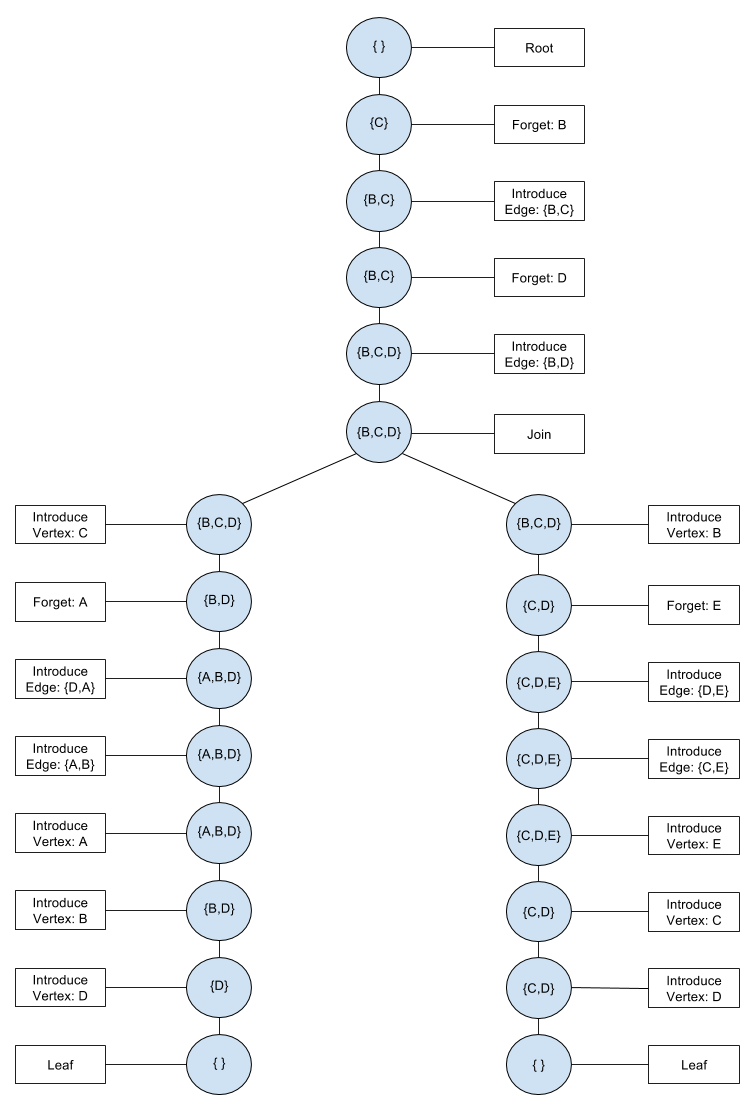
\includegraphics[width=1.0\textwidth]{./imgs/TD_3.png}
  	\caption{Eine Nice Tree Decomposition für den Ursprungsgraphen in Abbildung \ref{fig:td_1}}
\end{figure}

Sei eine Tree Decomposition gegeben, kann eine standardmäßige Nice Tree Decomposition von gleicher Breite in polynomieller Zeit gefunden werden \cite{kloks1994}. Der Algorithmus für eine standardmäßige Nice Tree Decomposition kann in der selben Laufzeit  modifizert werden, so dass das Ergebnis zusätzlich die o.g. Kriterien erfüllt.
\end{definition}

